\begin{Lema}\label{Lema:Disco_menos_puntos_retracto_de_plano_menos_puntos}
Para cualquier $n\in\mathbb{Z}^+$ tomamos $p_1,\dots,p_n\in B_1(0)$ distintos. Entonces $D^2\setminus\{p_1,\dots,p_n\}$ es un retracto de deformación de $\mathbb{R}^2\setminus\{p_1,\dots,p_n\}$.
\end{Lema}
\begin{proof}
Tomemos $X_1=\mathbb{R}^2\setminus B_1(0)=\{(x,y)\in\mathbb{R}^2\mid\lVert(x,y)\rVert\geq1\}$ y $X_2=D^2\setminus\{p_1,\dots,p_n\}$. Como $X_1\overset{\text{cer}}{\subseteq}\mathbb{R}^2$ y $X_1\subseteq\mathbb{R}^2\setminus\{p_1,\dots,p_n\}$, entonces $X_1\overset{\text{cer}}{\subseteq}\mathbb{R}^2\setminus\{p_1,\dots,p_n\}$. Como $X_2=D^2\cap\left( \mathbb{R}^2\setminus\{p_1,\dots,p_n\} \right)$ y $D^2\overset{\text{cer}}{\subseteq}\mathbb{R}^2$ entonces $X_2\overset{\text{cer}}{\subseteq}\mathbb{R}^2\setminus\{p_1,\dots,p_n\}$. Así, $X_1\times I\overset{\text{cer}}{\subseteq}(\mathbb{R}^2\setminus\{p_1,\dots,p_n\})\times I$ y $X_2\times I\overset{\text{cer}}{\subseteq}(\mathbb{R}^2\setminus\{p_1,\dots,p_n\})\times I$, y, como $X_1\cup X_2=\mathbb{R}^2\setminus\{p_1,\dots,p_n\}$ y $X_1\cap X_2=S^1$ entonces $(X_1\times I)\cup(X_2\times I)=(\mathbb{R}^2\setminus\{p_1,\dots,p_n\})\times I$, y $(X_1\times I)\cap(X_2\times I)=S^1\times I$. Definimos
\begin{align*}
H_1:X_1\times I&\longrightarrow\mathbb{R}^2\setminus\{p_1,\dots,p_n\}\\
(z,t)&\longmapsto\frac{z}{\lVert z\rVert}t+(1-t)z\\
H_2:X_2\times I&\longrightarrow\mathbb{R}^2\setminus\{p_1,\dots,p_n\}\\
(z,t)&\longmapsto z.
\end{align*}
Notemos que para cualquier $(z,t)\in X_1\times I$ se tiene $\lVert z\rVert\geq1$, y
\begin{align*}
\left\lVert\frac{z}{\lVert z\rVert}t+(1-t)z\right\rVert&=\left\lVert z\left(\frac{t}{\lVert z\rVert}+1-t\right)\right\rVert\\
&=\lVert z\rVert\left|\frac{t}{\lVert z\rVert}+1-t\right|\\
&=\left|t+(1-t)\lVert z\rVert\right|\\
&=t+(1-t)\lVert z\rVert\\
&=\left(t-1+(1-t)\lVert z\rVert\right)+1\\
&=(1-t)\left(\lVert z\rVert-1\right)+1\\
&\geq1,
\end{align*}
pues $1-t\geq0$ y $\lVert z\rVert-1\geq0$. Por tanto $\frac{z}{\lVert z\rVert}t+(1-t)z\notin\{p_1,\dots,p_n\}$, de modo que $H_1$ está bien definida. Como se obtiene a partir de funciones continuas mediante operaciones que preservan la continuidad, se tiene que $H_1$ es continua; como $H_2$ también es continua y para todo $(z,t)\in S^1\times I$ se tiene $H_1(z,t)=\frac{z}{\lVert z\rVert}t+(1-t)z=z=H_2(z,t)$, entonces, por el lema de pegado, la función
\begin{align*}
H:(\mathbb{R}^2\setminus\{p_1,\dots,p_n\})\times I&\longrightarrow\mathbb{R}^2\setminus\{p_1,\dots,p_n\}\\
(z,t)&\longmapsto H(z,t)=
\begin{cases}
H_1(z,t) & \text{si } z\in X_1\\
H_2(z,t) & \text{si } z\in X_2
\end{cases}
\end{align*}
es continua. Además,
\begin{itemize}
\item Para cualquier $z\in\mathbb{R}^2\setminus\{p_1,\dots,p_n\}$ tenemos
\begin{align*}
H(z,0)&=H_1(z,0)=z &&\text{si } z\in X_1,\\
H(z,0)&=H_2(z,0)=z &&\text{si } z\in X_2,\\
H(z,1)&=H_1(z,1)=\frac{z}{\lVert z\rVert}\in S^1\subseteq X_2 &&\text{si } z\in X_1,\\
H(z,1)&=H_2(z,1)=z\in X_2 &&\text{si } z\in X_2.
\end{align*}
\item Para cualesquiera $z\in X_2$ y $t\in I$ se tiene $H(z,t)=H_2(z,t)=z$.
\end{itemize}
Por tanto $X_2=D^2\setminus\{p_1,\dots,p_n\}$ es un retracto de deformación de $\mathbb{R}^2\setminus\{p_1,\dots,p_n\}$.
\end{proof}

\begin{Lema}\label{Lema:Rectangulo_menos_puntos_retracto}
Sea $n\in\mathbb{Z}^+$ y sean $p_1,\dots,p_n$ puntos distintos de $(-1,0)\times(-1,1)$. Sea $\varepsilon>0$ cualquiera y tomemos $X=([-1,\varepsilon)\times[-1,1])\setminus\{p_1,\dots,p_n\}$. Entonces $X_1=([-1,0]\times[-1,1])\setminus\{p_1,\dots,p_n\}$ es un retracto de deformación de $X$.
\end{Lema}
\begin{center}
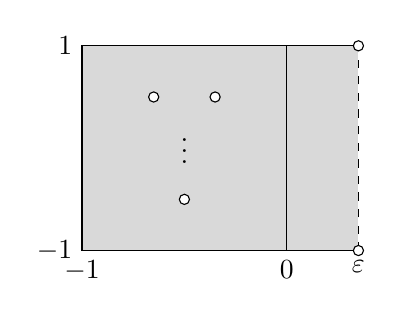
\begin{tikzpicture}[x=2.6cm,y=1.3cm,hole/.style={circle,draw,fill=white,inner sep=1.3pt}]
\fill[gray,opacity=0.3] (-1,-1) rectangle (0.35,1);
\draw (-1,-1) rectangle (0,1);
\draw (0,1) -- (0.35,1);
\draw (0,-1) -- (0.35,-1);
\draw[dashed] (0.35,-1) -- (0.35,1);
\node[hole] at (-0.65,0.5) {};
\node[hole] at (-0.35,0.5) {};
\node[inner sep=0pt] at (-0.5,0.05) {$\vdots$};
\node[hole] at (-0.5,-0.5) {};
\node[hole] at (0.35,1) {};
\node[hole] at (0.35,-1) {};
\node[left] at (-1,1) {$1$};
\node[left] at (-1,-1) {$-1$};
\node[below] at (-1,-1) {$-1$};
\node[below] at (0,-1) {$0$};
\node[below] at (0.35,-1) {$\varepsilon$};
\end{tikzpicture}
\end{center}
\begin{proof}
Tomemos $X_2=[0,\varepsilon)\times[-1,1]$. Notemos que $X_1\cup X_2=X$, $X_1=([-1,0]\times[-1,1])\cap X$ y $X_2=([0,\varepsilon]\times[-1,1])\cap X$. Como $[-1,0]\times[-1,1]$ y $[0,\varepsilon]\times[-1,1]$ son cerrados de $\mathbb{R}^2$ entonces $X_1$ y $X_2$ son cerrados de $X$. Tenemos $X_1\cap X_2=\{0\}\times[-1,1]$. De esta forma, $X_1\times I\overset{\text{cer}}{\subseteq}X\times I$, $X_2\times I\overset{\text{cer}}{\subseteq}X\times I$, $(X_1\times I)\cup(X_2\times I)=X\times I$, y $(X_1\times I)\cap(X_2\times I)=(\{0\}\times[-1,1])\times I$. Definimos las funciones
\begin{align*}
H_1:X_1\times I&\to X\\
((x,y),t)&\mapsto(x,y)\\
H_2:X_2\times I&\to X\\
((x,y),t)&\mapsto((1-t)x,y)
\end{align*}
que son continuas. Para cualesquiera $y\in[-1,1]$ y $t\in I$ se tiene $H_1((0,y),t)=(0,y)=H_2((0,y),t)$. Así, por el lema de pegado la función
\begin{align*}
H:X\times I&\to X\\
((x,y),t)&\mapsto
\begin{cases}
H_1((x,y),t) & \text{si } (x,y)\in X_1\\
H_2((x,y),t) & \text{si } (x,y)\in X_2
\end{cases}
\end{align*}
es continua. Además
\begin{itemize}
\item Para cualquier $(x,y)\in X$ se tiene
\begin{align*}
H((x,y),0)&=H_1((x,y),0)=(x,y) &&\text{si } (x,y)\in X_1,\\
H((x,y),0)&=H_2((x,y),0)=(x,y) &&\text{si } (x,y)\in X_2,\\
H((x,y),1)&=H_1((x,y),1)=(x,y)\in X_1 &&\text{si } (x,y)\in X_1,\\
H((x,y),1)&=H_2((x,y),1)=(0,y)\in X_1 &&\text{si } (x,y)\in X_2.
\end{align*}
\item Para cualesquiera $(x,y)\in X_1$ y $t\in I$ se tiene $H((x,y),t)=H_1((x,y),t)=(x,y)$.
\end{itemize}
Por tanto $X_1$ es un retracto de deformación de $X$.
\end{proof}

\begin{Lema}\label{Lema:Pi1_circulo_disco_menos_origen}
Para cualquier $z\in S^1$, $\pi_1(S^1,z)\cong\pi_1(D^2\setminus\{0\},z)$.
\end{Lema}
\begin{proof}
Por el \Cref{Lema:Esfera_retracto_de_Rn_menos_origen}, $S^1$ es un retracto de deformación de $\mathbb{R}^2\setminus\{0\}$, luego $\pi_1(S^1,z)\cong\pi_1(\mathbb{R}^2\setminus\{0\},z)$. Por el \Cref{Lema:Disco_menos_puntos_retracto_de_plano_menos_puntos}, $D^2\setminus\{0\}$ es un retracto de deformación de $\mathbb{R}^2\setminus\{0\}$, luego $\pi_1(D^2\setminus\{0\},z)\cong\pi_1(\mathbb{R}^2\setminus\{0\},z)$. Obtenemos que $\pi_1(S^1,z)\cong\pi_1(D^2\setminus\{0\},z)$.
\end{proof}
\textbf{e)} Tome dos puntos distintos $p,q\in\mathbb{R}^2$ y considere el espacio $\mathbb{R}^2-\{p,q\}$, cuál es su grupo fundamental.
\begin{proof}[\textbf{Solución}]
Sin pérdida de generalidad podemos tomar $p=(-\tfrac12,0)$ y $q=(\tfrac12,0)$. Por el \Cref{Lema:Disco_menos_puntos_retracto_de_plano_menos_puntos}, $D^2\setminus\{p,q\}$ es un retracto de deformación de $\mathbb{R}^2\setminus\{p,q\}$, luego $\pi_1(\mathbb{R}^2\setminus\{p,q\},0)\cong\pi_1(D^2\setminus\{p,q\},0)$, y $D^2\setminus\{p,q\}\cong Y:=([-1,1]\times[-1,1])\setminus\{p,q\}$. Llamando $O_1$ a la imagen de $0$ bajo el homeomorfismo, se tiene $\pi_1(D^2\setminus\{p,q\},0)\cong\pi_1(Y,O_1)$. Como $Y$ es conexo por caminos, $\pi_1(Y,O_1)\cong\pi_1(Y,0)$. Tomemos $U=([-1,\tfrac14)\times[-1,1])\setminus\{p\}$ y $V=((-\tfrac14,1]\times[-1,1])\setminus\{q\}$. Como $U=((-2,\tfrac14)\times(-2,2))\cap Y$ y $V=((-\tfrac14,2)\times(-2,2))\cap Y$ con $(-2,\tfrac14)\times(-2,2)$ y $(-\tfrac14,2)\times(-2,2)$ abiertos de $\mathbb{R}^2$, entonces $U\subseteqab Y$ y $V\subseteqab Y$. Además $Y=U\cup V$; $U$, $V$ y $U\cap V=(-\tfrac14,\tfrac14)\times[-1,1]$ son conexos por caminos, y $U\cap V$ es simplemente conexo, pues es convexo y por tanto estrellado. De esta manera, por el corolario del Teorema de Seifert-Van Kampen se tiene $\pi_1(Y,0)\cong\pi_1(U,0)*\pi_1(V,0).$
\begin{center}
\begin{tikzpicture}[x=2.2cm,y=1.1cm,
hole/.style={circle,draw,fill=white,inner sep=1.3pt},
lab/.style={font=\small}]
% Figura de U
\begin{scope}
\fill[gray,opacity=0.3] (-1,-1) rectangle (0.25,1);
\draw (-1,-1) rectangle (0,1);
\draw (0,1) -- (0.25,1);
\draw (0,-1) -- (0.25,-1);
\draw[dashed] (0.25,-1) -- (0.25,1);
\node[hole] at (0.25,1) {};
\node[hole] at (0.25,-1) {};
\node[hole,label={[lab]below:$p$}] at (-0.5,0) {};
\node[lab,left] at (-1,1) {$1$};
\node[lab,left] at (-1,-1) {$-1$};
\node[lab,below] at (-1,-1) {$-1$};
\node[lab,below] at (0,-1) {$0$};
\node[lab,below] at (0.25,-1) {$\tfrac14$};
\node at (-0.375,-1.7) {$U$};
\end{scope}
% Figura de V
\begin{scope}[xshift=3.4cm]
\fill[gray,opacity=0.3] (-0.25,-1) rectangle (1,1);
\draw (0,-1) rectangle (1,1);
\draw (-0.25,1) -- (0,1);
\draw (-0.25,-1) -- (0,-1);
\draw[dashed] (-0.25,-1) -- (-0.25,1);
\node[hole] at (-0.25,1) {};
\node[hole] at (-0.25,-1) {};
\node[hole,label={[lab]below:$q$}] at (0.5,0) {};
\node[lab,right] at (1,1) {$1$};
\node[lab,right] at (1,-1) {$-1$};
\node[lab,below] at (1,-1) {$1$};
\node[lab,below] at (0,-1) {$0$};
\node[lab,below left] at (-0.25,-1) {$-\tfrac14$};
\node at (0.375,-1.7) {$V$};
\end{scope}
\end{tikzpicture}
\end{center}
Por el \Cref{Lema:Rectangulo_menos_puntos_retracto} tenemos que $W=([-1,0]\times[-1,1])\setminus\{p\}$ es un retracto de deformación de $U$, luego $\pi_1(U,0)\cong\pi_1(W,0)$. Como $W\cong D^2\setminus\{0\}$, siendo $O_2$ la imagen de $0$ bajo el homeomorfismo, tenemos $\pi_1(W,0)\cong\pi_1(D^2\setminus\{0\},O_2)$. Como $D^2\setminus\{0\}$ es conexo por caminos, se tiene $\pi_1(D^2\setminus\{0\},O_2)\cong\pi_1(D^2\setminus\{0\},(0,1))$ y por el \Cref{Lema:Pi1_circulo_disco_menos_origen}, $\pi_1(D^2\setminus\{0\},(0,1))\cong\pi_1(S^1,(0,1))\cong(\mathbb{Z},+)$. Por la transitividad de $\cong$ tenemos $\pi_1(U,0)\cong(\mathbb{Z},+)$. Como $U\cong V$ mediante una función que deja fijo a $0$, tenemos $\pi_1(U,0)\cong\pi_1(V,0)$, luego $\pi_1(V,0)\cong(\mathbb{Z},+)$ y con esto $\pi_1(Y,0)\cong(\mathbb{Z},+)*(\mathbb{Z},+)$. Por la transitividad de $\cong$, $\pi_1(\mathbb{R}^2\setminus\{p,q\},0)\cong(\mathbb{Z},+)*(\mathbb{Z},+)$. Como $\mathbb{R}^2\setminus\{p,q\}$ es conexo por caminos, para cualquier $z\in\mathbb{R}^2\setminus\{p,q\}$ se tiene $\pi_1(\mathbb{R}^2\setminus\{p,q\},z)\cong\pi_1(\mathbb{R}^2\setminus\{p,q\},0)$ y por tanto $\pi_1(\mathbb{R}^2\setminus\{p,q\},z)\cong(\mathbb{Z},+)*(\mathbb{Z},+)$.
\end{proof}
